\chapter{Inverse Function Theorem}
\dfnc{Homeomorphism}{A bijective continuous function whose inverse  is also continuous  is called homeomorphism}


\begin{theorem}{Inverse Function Theorem}{invthm}
	Suppose $U$ be an open set in $\bbR^n$. $f:U\to \bbR^n$ be a $C^1$ function. $f'(a)=A$ is invertible . Then \begin{enumerate}[label=\bfseries\tiny\protect\circled{\small\arabic*}]
	\item $f$ is injective in some neighborhood of $a$
	\item There are open sets $V\subset U, a\in V$ and $W\subset \bbR^n, f(a)\in W$ such that $f$ is a bijection $V\mathrel{\raisebox{2pt}{$\xrightarrow{f}$}
		\llap{\raisebox{-2pt}{$\xleftarrow[g]{}$}}}W$ whose inverse, $g$ is also continuous i.e. a local homeomorphism  i.e. at the given point $a$  there exists a neighborhood  at which $f$ is homeomorphism
	\item $f^{-1}$ is also differentiable  on $W$  i.e. for any $f(u)\in W$ $$Df^{-}(f(u))=Df(u)^{-1}$$
\end{enumerate}
\end{theorem}
\nt{\begin{enumerate}
		\item \textbf{Crucial} that $\dim U$ and target  are the same
		\item There are appropriate versions of the theorem when $f'(a)$ is injective / surjective / arbitrary (when $f'(a)$ is surjective it is the Implicit Function Theorem) those versions can be proved using the theorem
	\end{enumerate}


}


\begin{proof}
	\begin{itemize}
		\item $n=1$ is easy. Directly using $MVT$
		\item We may assume  that $a=0$  and $f(a)=0$ (replace $f$ by $f(u+a)-f(a)$) and $f'(a)=$ Identity (replace $f$ by $f'(a)^{-1}f(a)$) check that the result  for given $f$ follows easily from result for this normalized $f$
		\parinn
		
		Normalization makes formulation / calculation  in the proof a bit simpler but may assume a  bit the natural main ideas, so we won't normalize.
	\end{itemize}
\begin{enumerate}[label=\bfseries\tiny\protect\circled{\small\arabic*}]
	\item Injectivity of $f$ on a ball $B$ around $a$ of small radius $\veps$. We will choose $\veps$ later.
	
	Best linear approximation for $f(x)$ near $a$ is $f(x)+f'(a)(x-a)$. If $f$ were = this function, the theorem is easy so let's examine the remainder \begin{align*}
		r(x) & = f(x)-f(a)-f'(a)(x-a)\\
		r'(x) & = f'(x)-f'(a)
	\end{align*}
We can make $f'(x)-f'(a)$ small in some ball $B$ around $a$ by continuity of $f'$ at  $a$. $$r(x_1)-r(x_2)=f(x_1)-f(x_2)-f'(a)(x_1-x_2)$$

Choose a good open ball $B$ centered at $a$ with all of the following properties:
\begin{enumerate}[label=(\roman*)]
	\item Ensure that $\forall \ x\in B$ $\|f'(x)-f'(a)\|<\veps$
	\item $U\xrightarrow{f}L(\bbR^n)\xrightarrow{\det}\bbR$ is continuous at $a$ and $\det f'(a)\neq 0$ so can choose $B$ such that $\forall\ x\in B$, $\det f'(x)\neq 0$ and hence $f(x)$ is invertible.
	\item Shrink $B$ further if necessary to ensure $\overline{B} \subset U$ (useful later to minimize a continuous function on this compact set.)
\end{enumerate}
\begin{center}
	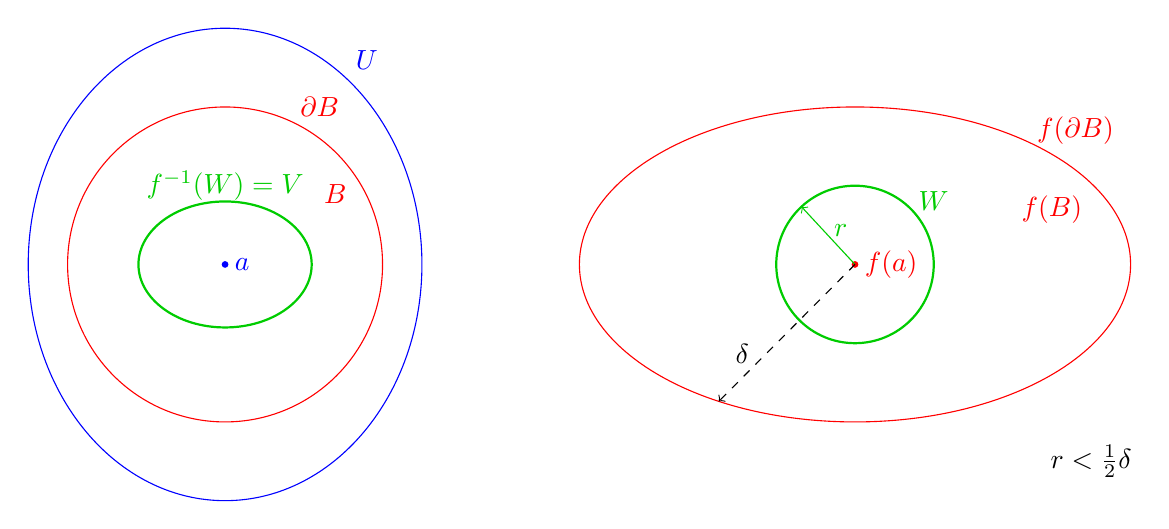
\begin{tikzpicture}
		\draw[red] (4,0) circle [x radius=3.5cm, y radius=2cm] node[xshift=2.8cm, yshift=1.7cm]{$f(\partial B)$} node[xshift=2.5cm, yshift=0.7cm]{$f(B)$} node[xshift=3cm,yshift=-2.5cm,black]{$r<\frac12\delta$};
		\draw[blue] (-4,0) circle [x radius=2.5cm, y radius=3cm] node[xshift=1.8cm, yshift=2.6cm]{$U$} ;
		\filldraw[blue] (-4,0) circle (1pt) node[anchor=west]{$a$};
		\filldraw[red] (4,0) circle (1pt) node[anchor=west]{$f(a)$};
		\draw[green!80!black,thick] (4,0) circle (1cm)  node[xshift=1cm,yshift=0.8cm]{$W$};
		\draw[green!80!black,thick] (-4,0) circle [x radius=1.1cm, y radius=0.8cm]node[xshift=0cm,yshift=1cm]{$f^{-1}(W)=V$};
		\draw[red] (-4,0) circle (2cm) node[xshift=1.2cm, yshift=2cm]{$\partial B$} node[xshift=1.4cm, yshift=0.9cm]{$ B$};
		\draw[green!80!black,->] (4,0) -- (3.32,0.733) node[xshift=5mm,yshift=-3mm] {$r$};
		\draw[dashed,->] (4,0) -- (2.27,-1.739) node[xshift=3mm, yshift=6mm]{$\delta$};
		
	\end{tikzpicture}
\end{center}
$\forall\ x\in B$ , $f'(x)$ is invertible. $\|r'(x)\|=\|f'(x)-f'(a)\|<\veps$. By $MVT$ applied on $r(x)$ on the convex set $B$, we get for any $x_1,x_2\in B$ $$\|f(x_1)-f(x_2)-f'(a)(x_1-x_2)\|=\|r(x_1)-r(x_2)\|\leq \veps \|x_1-x_2\|$$Now recall $\|p-q\|\geq \|p\|-\|q\|$. Hence $$\|f(x_1)-f(x_2)-f'(a)(x_1-x_2)\|\geq \|f'(a)(x_1-x_2)\|-\|f(x_1)-f(x_2)\|$$\textbf{Upshot: }$\|f(x_1)-f(x_2)\|\geq \|f'(a)(x_1-x_2)\|-\veps\|x_1-x_2\|\geq \overset{\substack{\text{Needed} \\ \downarrow}}{\cdots}$
\nt{At this point if we had normalized $f'(a)=$ Identity then we would have gotten $$\|f(x_1)-f(x_2)\|\geq (1-\veps)\|x_1-x_2\|$$ Taking $\veps<1$ fives the injectivity of $f$}\parinn

In our case we need to find lower bound on $\|f'(a)(x_1-x_2)\|$. Minimize $\{\|f'(a)u\|\mid \|u\|=1\}$. $f'(a)$ is continuous and the set of all unit vectors is compact. This set has a minimum, minimum=$m>0$ as it is invertible so $f'(\text{non zero vector})\neq 0$. 

Now take $\veps<m$ and then in the resulting ball $B$ we have \begin{equation}
	\|f(x_1)-f(x_2)\|\geq (m-\veps)\|x_1-x_2\|\label{eq1}
\end{equation}This gives the injectivity of $f$ on $B$. So we have the bijection $B\mathrel{\raisebox{2pt}{$\xrightarrow{\ \ \  f\ \ \ }$}
\llap{\raisebox{-2pt}{$\xleftarrow[f^{-1}=g]{}$}}}f(B)$. \eqref{eq1} is saying that any $y_1=f(x_1), y_2=f(x_2)$ in $f(B)$, i.e. $g(y_1)=x_1,g(y_2)=x_2$ $$\|g(y_1)-g(y_2)\|\leq \frac{1}{m-\veps}\|y_1-y_2\|$$ i.e. $g$ is uniformly continuous.

\item We have bijection of $f$ between $B$ and $f(B)$, $V$ is supposed to be open but we have taken open ball, so its open. Inverse of $f$ ($g$) is continuous so what left is $f(B)$ open\parinn

To show that $f$ is a local Homeomorphism it is enough to find an open ball $W$ around $f(a)$ with $W\subset f(B)$. Then we simply take $V=f^{-1}(W)$ which is open by continuity of $f$ and clearly $V\mathrel{\raisebox{2pt}{$\xrightarrow{f}$}
	\llap{\raisebox{-2pt}{$\xleftarrow[g]{}$}}}W$ are bijections just restrict $f,g$ from $B,f(B)$ respectively.

How to construct $W$? What radius to take around $W$? Stay away from $f(\partial B)$. $\delta=\min\{ \|f(x)-f(a)\| \mid x\in \partial B  \}>0$. Choose radius of $W$ to be $\frac12\delta$. We will be done if we show $W\subset f(B)$ i.e. given any $c\in W$ $\exs\ x^*\in B$ such that $f(x^*)=c$ ($x^*$ is necessarily unique, by injectivity).\parinf

\textbf{\textit{Idea: }}Consider the differentiable function $\begin{cases}
	B\to \bbR_{\geq 0}\\ x\mapsto \|f(x)-c\|^2
\end{cases}$\parinn


Note that $\|c-\text{ any point on }f(\partial B)\|>r$ by triangle inequality where as $\|c-f(a)\|<r$ (as $c$ is inside $W=$ ball of radius $r<\frac12\delta$ around $f(a)$). Hence $\|f(x)-c\|^2$ will take its minimum value at some point say $x^*\in B$. Now $f=(f_1,f_2,\dots,f_n)$ and $c=(c_1,\dots,c_n)$ $$\mu(x)=\|f(x)-c\|^2=\sum_{i=1}^n (f_i(x)-c_i)^2$$Derivative of this function is $0$ at $x^*$

\begin{center}
	\begin{tikzcd}
		B \arrow[r, "f"] & \bbR^n \arrow[ r, "\mu"] & \bbR \\
		x \arrow[r, maps to] & f(x)=y \arrow[r, maps to] & \|y-c\|^2
	\end{tikzcd}
\end{center}
Hence $$\EqM{c1}{\underbrace{\mu'(f(x^*))}}\circ f'(x^*)=0$$
\begin{tikzpicture}[remember picture, 
	overlay
	]
	\draw[<-] ++(c1.south) -- ++(0,-2em)  node[xshift=-1.6cm,yshift=-.6cm] {$\mat{2(f_1(x^*)-c_1) & \cdots & 2(f_n(x^*)-c_n)}$ (Matrix of $f'(x^*)$ -- Invertible) };
\end{tikzpicture}

\vspace{1.5cm}

Therefore $\mat{2(f_1(x^*)-c_1) & \cdots & 2(f_n(x^*)-c_n)}$ must be 0 i.e. $f_i(x^*)=c_i$ i.e. $f(x^*)=c$. So we showed that each $c\in W$ is in the image of $f$. Now take $V=f^{-1}(W)$ and we have the Homeomorphism.


\item Differentiability of $f^{-1}=g$ at any point $y\in W$.

\begin{center}
	\begin{tikzcd}
		x \arrow[r, rightharpoonup, "f",yshift=0.5mm] \arrow[d, bend right=25,"\text{add }h", swap] & y \arrow[l, rightharpoonup, "g", yshift=-0.5mm] \arrow[d, bend left=25, "\text{add }k"]  \\
		x+h \arrow[r, rightharpoonup, "f",yshift=0.5mm] & y+k\in W \arrow[l, rightharpoonup, "g", yshift=-0.5mm]
	\end{tikzcd}
\end{center}

Take small $k\in\bbR^n$ and let $h=g(y+k)-g(y)$ and $k=f(x+h)-f(x)$. Each of $h$ and $k$ determines the other uniquely. In particular $h\neq 0\iff k\neq 0$ (by bijectivity). $h\to 0 \iff k\to 0$ (by continuity of $f$ and $g$). $\alpha(h)=f(x+h)-f(x)-Th=k-Th$ where $T=f'(x)$. Then we have $\frac{\|\alpha(h)\|}{\|h\|}\to 0$ as $\|h\|\to 0$. We want to show $g'(y)=T^{-1}$

Let $\beta(k)=g(y+k)-g(y)-T^{-1}k=h-T^{-1}k$. We will show that as $k\to 0$, $\frac{\|\beta(k)\|}{\|k\|}\to 0$\begin{align*}
	\frac{\|\beta(k)\|}{\|k\|} = \frac{\|h-T^{-1}k\|}{\|k\|}= \frac{\|T^{-1}(Th-k)\|}{\|k\|} & \leq \frac{\|T^{-1}\|}{\|k\|}\|Th-k\|\\
	& = \frac{\|T^{-1}\|}{\|k\|} \|\alpha(h)\|\\
	& = \frac{\|T^{-1}\|}{\|k\|} \frac{\|\alpha(h)\|}{\|h\|}\|h\|\\
	& = \|T^{-1}\|\frac{\|h\|}{\|k\|}  \frac{\|\alpha(h)\|}{\|h\|}
\end{align*}
We know by $\frac{\|h\|}{\|k\|} <\frac{1}{m-\veps}$ by  \eqref{eq1}. $\frac{\|\alpha(h)\|}{\|h\|}\to 0$ as $k\to 0$ because then $h\to 0$.
\end{enumerate}
\end{proof}
\nt{\begin{itemize}
		\item For another proof of surjectivity onto $W$, see Rudin's use of contraction property
		\item There is a more general result which assumed only invertibility of $f'(x)$ for $x\in U$ but not continuity of $f'$ everywhere. (See exposition on Terence Tao's Blog: \url{https://terrytao.wordpress.com/tag/inverse-function-theorem/})
		\item $f$ need not be globally invertible!
		
		Example = See Problem 17 from Rudin
		
		$f(x,y)=(e^x\cos y,e^x\sin y)$. Then $$f'(x,y)=\mat{e^x\cos y & -e^x\sin y\\ e^x\sin y & e^x\cos y}\xrightarrow{\det}(e^x)^2(\cos^2x+\sin^2y)=e^{2x}>0$$Thus $f$ is locally invertible everywhere with $C^{1}$ inverse.
		\item $f$ is not globally one-one $f(x,y)=f(x,y+2\pi)$. Do the rest.
\end{itemize}}
\corc{}{If $f$ is a $C^1$ map from open $U$ in $\bbR^n$ to $\bbR^n$ and $f'(x)$ is invertible $\forall\ x\in U$ then\begin{enumerate}[label=\bfseries\tiny\protect\circled{\small\arabic*}]
		\item $f$ is an open map 
		\item $f$ is locally invertible with each such inverse a $C^1$ dunction (because matrix of $(f^{-1})'=$ inverse of matrix of $f'$ and entries of $A^{-1}=\frac1{\det A}$ (polynomials in entries of $A$) in particular $A\to A^{-1}$ is continuous)
\end{enumerate}}
